\begin{abstract}
Voltage acquisition requires a numerical conversion, an electrical calibration and a defined circuit load. Microcontroller inputs and an external multimeter expose these requirements in different forms. A six-level multimeter staircase gives a gain of 1.001995 and an offset of $0.504\unit{mV}$ relative to nominal example settings; raw and displayed values agree under the defined numerical conversion. In the independent microcontroller example, capacitor charging and discharging give time constants of 0.9997 and $0.9995\unit{s}$. A common affine voltage error changes fitted amplitudes and asymptotes while preserving this timescale, whereas timebase error or loading can alter its physical interpretation. Granularity, calibration covariance and circuit dynamics must therefore be assessed at the stage where each affects the inferred quantity.
\end{abstract}
\begin{IEEEkeywords}
Voltage measurement, ADC, digital multimeter, calibration, loading, RC circuits.
\end{IEEEkeywords}

\section{A shared measurement chain}
A converter code or a Bluetooth notification becomes a voltage indication only after scale, sign and units have been assigned. Physical voltage measurement then requires an independently checked transfer relation and a circuit whose operating point is not changed unknowingly by the readout. The same distinction applies to a microcontroller input and a digital multimeter, even though their resolutions, input circuits and conversion timing differ.

For an ADC code $q$, write an affine indication
\begin{equation}
 U_d=a+bq.
 \label{eq:analog-inputs-transfer}
\end{equation}
A multimeter notification instead represents a signed displayed number together with function, decimal scaling and a unit prefix. Recovering that number correctly verifies the representation. It does not determine the electrical gain or offset at the terminals. Conversely, a calibrated meter does not guarantee that an unrecognised range or packet format will be interpreted correctly.

The examples are used for different tests. The Nano's A0 potentiometer sweep checks a broad code interval, A1 follows a light-dependent circuit, and A2 provides charging and discharging branches. The Owon staircase supplies repeated positive, zero and negative plateaux for a signed affine reduction. The Nano record uses device timestamps and the multimeter uses Bluetooth receive times. The runs compare numerical granularity across the two acquisition paths.

\section{Calibration at the terminals and loading in the circuit}
\begin{figure}[t]
\centering
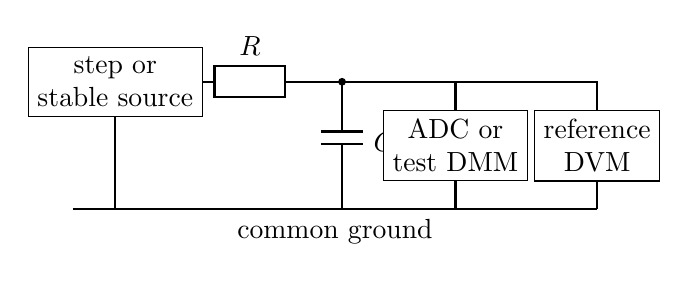
\begin{tikzpicture}[x=0.9cm,y=0.9cm]
 \node[draw,align=center] (src) at (0.6,0.8) {step or\\stable source};
 \draw[thick] (src.east)--(2.0,0.8);
 \draw[thick] (2.0,0.58) rectangle (3.0,1.02);
 \node at (2.5,1.3) {$R$};
 \draw[thick] (3.0,0.8)--(6.8,0.8);
 \fill (3.8,0.8) circle (0.055);
 \draw[thick] (3.8,0.8)--(3.8,0.1);
 \draw[thick] (3.5,0.1)--(4.1,0.1);
 \draw[thick] (3.5,-0.08)--(4.1,-0.08);
 \draw[thick] (3.8,-0.08)--(3.8,-1.0);
 \node at (4.4,-0.05) {$C$};
 \node[draw,fill=white,align=center] (dut) at (5.4,-0.1) {ADC or\\test DMM};
 \node[draw,fill=white,align=center] (ref) at (7.4,-0.1) {reference\\DVM};
 \draw[thick] (5.4,0.8)--(dut.north);
 \draw[thick] (6.8,0.8)--(7.4,0.8)--(ref.north);
 \draw[thick] (0,-1.0)--(7.4,-1.0);
 \draw[thick] (dut.south)--(5.4,-1.0);
 \draw[thick] (ref.south)--(7.4,-1.0);
 \draw[thick] (src.south)--(0.6,-1.0);
 \node[below] at (3.7,-1.0) {common ground};
\end{tikzpicture}
\caption{Calibration and RC apparatus. A reference DVM observes the same terminals as the test readout. For a capacitor transient, all input paths load the capacitor node; their parallel resistance enters the dynamic model.}
\label{fig:analog-inputs-apparatus}
\end{figure}

Apply several independently known voltages to each channel, including interior levels and both polarities where the input permits them. Interleave a repeated level and reverse the sweep to distinguish drift from nonlinearity. Keep source resistance, input impedance, range and settling conditions in the calibration record. The reference must observe the same terminals as the instrument under test, not merely another nominally equal source setting.

The Nano's nRF52840 has a successive-approximation ADC with configurable reference, gain and acquisition time~\cite{nrf52840}. The board-core acquisition requests ten-bit results~\cite{arduinocore}; requested output width and physical converter capability are distinct~\cite{analogread}. The example uses $3.226\unit{mV/count}$, close to the endpoint convention $3300/1023$, whereas a 3.3-V, ten-bit bin width is $3300/1024=3.2227\unit{mV}$. Neither convention establishes the actual reference voltage or terminal scale.

An ADC acquires charge on an internal sampling capacitor. Source resistance and acquisition time determine settling, particularly after switching from another channel at a different potential~\cite{nrf52840}. The three channels are sequentially acquired at approximately 20 Hz; a common frame time does not establish simultaneous conversion for phase measurements. The supply rails constrain allowable pin voltage independently of the numerical conversion scale.

For the Owon B35T's 6.000-V DC range, one display digit is $1\unit{mV}$. The specified limit $\pm(0.5\%\text{ of reading}+2\text{ digits})$ corresponds to $\pm7\unit{mV}$ at 1.000 V~\cite{owon35}. This manufacturer limit is much larger than the scatter of the example plateau means. It applies under the manual's conditions and is not an uncertainty assigned solely from a stable sequence of repeated digits.

Loading has to be included in the physical model. A photocell observed across a shunt $R_s$ and meter input $R_m$ supplies
\begin{equation}
 I=U(R_s^{-1}+R_m^{-1}).
 \label{eq:analog-inputs-shunt}
\end{equation}
The burden voltage must remain within the intended current-source operating region. Open-circuit cell voltage and loaded photocurrent do not have the same relation to illumination. Correct decoding cannot remove this electrical change in operating point.

\section{The signed reference staircase}
Figure~\ref{fig:analog-inputs-records} contrasts the circuit transient and the independent multimeter staircase. The meter sequence has nominal levels 0, 1.0, 1.5, 2.0, $-1.0$ and 0.5 V. Exclude the first and last second of each ten-second level, leaving 16 readings per plateau. Every interval below includes its lower endpoint and excludes its upper endpoint.

\begin{figure}[t]
\centering
% Two independent electrical records; horizontal positions are not paired.
\begin{tikzpicture}
\begin{groupplot}[group style={group size=1 by 2,vertical sep=1.2cm},
 width=0.97\columnwidth,height=3.6cm,
 grid=major,enlarge x limits=false,
 legend style={font=\scriptsize,at={(0.5,1.03)},anchor=south,
 legend columns=3,draw=none,fill=none},
 title style={font=\scriptsize,at={(0.02,0.97)},anchor=north west,fill=white},
 label style={font=\footnotesize},tick label style={font=\scriptsize}]
\nextgroupplot[ylabel={ADC display (V)},xlabel={ADC device time (s)},title={(a) Three circuit channels}]
\addplot[csblue,line width=0.7pt] table[col sep=comma,x=c0,y expr={0.001*\thisrow{c4}}] {data/analog_input_plot_v1-2.csv};
\addlegendentry{A0}
\addplot[csred,dashed,line width=0.7pt] table[col sep=comma,x=c0,y expr={0.001*\thisrow{c5}}] {data/analog_input_plot_v1-2.csv};
\addlegendentry{A1}
\addplot[csteal,dashdotted,line width=0.7pt] table[col sep=comma,x=c0,y expr={0.001*\thisrow{c6}}] {data/analog_input_plot_v1-2.csv};
\addlegendentry{A2}
\nextgroupplot[ylabel={DMM display (V)},xlabel={DMM receive time (s)},title={(b) Signed staircase}]
\addplot[csblue,line width=0.7pt,mark=*,mark size=0.65pt] table[col sep=comma,x=c0,y=c1] {data/owon_digital_multimeter-debug.csv};
\end{groupplot}
\end{tikzpicture}

\caption{Indicated voltages on each record's own clock: (a) ADC channels A0 (potentiometer), A1 (light-dependent circuit) and A2 (capacitor); (b) the independent multimeter's signed DC-voltage staircase.}
\label{fig:analog-inputs-records}
\end{figure}

\begin{table}[t]
\caption{Interior multimeter plateau means and deviations from nominal voltage levels.}
\label{tab:analog-inputs-staircase}
\centering\small
\begin{tabular}{@{}rrrr@{}}
\toprule
Window (s) & Nominal (V) & Mean (V) & Deviation (mV)\\
\midrule
1--9 & 0.0 & 0.00050 & 0.500\\
11--19 & 1.0 & 1.00250 & 2.500\\
21--29 & 1.5 & 1.50338 & 3.375\\
31--39 & 2.0 & 2.00450 & 4.500\\
41--49 & $-1.0$ & $-1.00156$ & $-1.562$\\
51--59 & 0.5 & 0.50169 & 1.687\\
\bottomrule
\end{tabular}
\end{table}

The raw numeric field on the selected range has a millivolt scale. Recalculation reproduces the indicated voltages, including the negative step, to floating-point rounding precision. This checks sign and numerical scaling independently of the nominal settings. Overload, an unknown prefix and the wrong meter interpretation are invalid states to reject, rather than small numerical errors to include in a calibration fit.

Fit the plateau means to $U_d=a+gU_{\rm nominal}$ by ordinary least squares. The result is $g=1.0019946$ and $a=0.5036\unit{mV}$, with maximum absolute plateau residual $0.1866\unit{mV}$. Within-plateau sample SDs range from 0.479 to $0.516\unit{mV}$. These quantities quantify the scale and offset relative to the stated levels. Repeated codes also do not independently sample every quantisation phase.

The Nano record illustrates the same distinction in a different form. All displayed voltages reproduce the stated count multiplication to numerical rounding precision. A0 spans codes 187--870, displayed as approximately 603--2807 mV, while A1 follows a slower light-dependent response. That response includes the external sensor circuit; conversion to an illumination scale depends on the circuit's calibration. The ADC display increment is 3.226 times the multimeter's 1-mV digit on the chosen range. This is a comparison of numerical granularity, not a measurement of either instrument's absolute accuracy.

\section{Circuit parameters that survive an affine scale}
The capacitor channel permits a shape-based inference despite an uncertain common voltage gain. Smartphone RC experiments use the same distinction between amplitude calibration and a physical timescale~\cite{torriente2023rc}. Fit each branch using actual recorded times and
\begin{equation}
 U(t)=U_\infty+A\exp[-(t-t_0)/\tau].
 \label{eq:analog-inputs-rc}
\end{equation}
The time origins are 5 s for charging and 35 s for discharge. For each trial positive $\tau$, estimate $A$ and $U_\infty$ by linear least squares, then minimise the residual sum of squares over $\tau$. With free amplitude, $t_0$ fixes the amplitude convention rather than introducing another independent shape parameter.

\begin{table}[t]
\caption{Exponential fits to capacitor charging and discharging. Residual RMS is $\sqrt{\mathrm{SSE}/N}$; $\tau$ is the fitted time constant.}
\label{tab:analog-inputs-rc}
\centering\small
\begin{tabular}{@{}lrr@{}}
\toprule
Quantity & Charging & Discharging\\
\midrule
Fit window (s) & 5--12 & 35--42\\
Observations & 139 & 139\\
$\tau$ (s) & 0.9997 & 0.9995\\
$U_\infty$ (mV) & 2995.4 & 1.7\\
Residual RMS (mV) & 1.76 & 1.91\\
\bottomrule
\end{tabular}
\end{table}

Shortening the windows to 5--10 and 35--40 s changes the two time constants by less than $0.2\unit{ms}$. This is an interval-sensitivity check, not a reference-clock or circuit-model uncertainty. A constant voltage offset and gain are absorbed into $U_\infty$ and $A$, leaving $\tau$ unchanged. Timebase scale error transfers directly into $\tau$, and input-dependent gain or additional relaxation processes can change its fitted value.

For the illustrated topology, the source remains connected through $R$ during both high and low states. With total parallel readout resistance $R_L$, the time constant is
\begin{equation}
 \tau=(R\parallel R_L)C,
 \qquad U_{\infty,\rm high}=U_s\frac{R_L}{R+R_L}.
 \label{eq:analog-inputs-loaded}
\end{equation}
Disconnecting the source instead of switching it low creates a different discharge circuit. An inferred capacitance therefore requires the actual switching topology, resistances and reference timing. Agreement of the example charging and discharging fits tests consistency within the exponential model, without identifying $R$, $C$ and loading separately.

\section{Uncertainty attached to the inferred quantity}
For a voltage correction, propagate reference uncertainty and the joint covariance of fitted offset and gain, together with drift, resolution and loading~\cite{gum}. A display step is a resolution statement. Under a uniform within-code model, the ADC's $3.226/\sqrt{12}=0.931\unit{mV}$ single-reading contribution does not decrease merely because identical codes are repeated. Avoid counting quantisation twice when repeatability already includes code fluctuations.

For a time constant, voltage-scale covariance is largely absorbed by the free amplitude and asymptote, but timebase uncertainty and circuit-model error remain. Residual structure near the step can indicate incomplete settling, leakage or an additional time constant. Repeat with another known resistance and check the predicted loaded scaling, rather than interpreting small residuals alone as validation.

Dynamic multimeter work additionally needs independently timed source transitions to establish conversion and delivery behaviour. Receive timestamps do not reveal the instrument's integration aperture. Thus the staircase establishes signed numerical consistency and an affine example reduction, while the RC trace identifies an approximately one-second relaxation under a stated model. The electrical reference, load and timing determine which further voltage or component claims those numbers can support.
